\documentclass[a4paper, 14pt]{extarticle}
\usepackage[russian]{babel}
\usepackage[T1]{fontenc}
\usepackage{fontspec}
\usepackage{indentfirst}
\usepackage{enumitem}
\usepackage{graphicx}
\usepackage[
  left=20mm,
  right=10mm,
  top=20mm,
  bottom=20mm
]{geometry}
\usepackage{parskip}
\usepackage{titlesec}
\usepackage{xurl}
\usepackage{hyperref}
\usepackage{float}
\usepackage[
  figurename=Рисунок,
  labelsep=endash,
]{caption}
\usepackage[outputdir=build, newfloat]{minted}

\hypersetup{
  colorlinks=true,
  linkcolor=black,
  filecolor=blue,
  urlcolor=blue,
}

\renewcommand*{\labelitemi}{---}
\setmainfont{Times New Roman}
\setmonofont{JetBrains Mono}[
  SizeFeatures={Size=11},
]

\newenvironment{code}{\captionsetup{type=listing}}{}
\SetupFloatingEnvironment{listing}{name=Листинг}

\setminted{
  fontsize=\footnotesize,
  frame=lines,
  framesep=2mm,
}

\setlength{\parskip}{6pt}

\setlength{\parindent}{1cm}
\setlist[itemize]{itemsep=0em,topsep=0em,parsep=0em,partopsep=0em,leftmargin=2.0cm,wide}
\setlist[enumerate]{itemsep=0em,topsep=0em,parsep=0em,partopsep=0em,leftmargin=2.0cm,wide}

\renewcommand{\thesection}{\arabic{section}.}
\renewcommand{\thesubsection}{\thesection\arabic{subsection}.}
\renewcommand{\thesubsubsection}{\thesubsection\arabic{subsubsection}.}

\titleformat{\section}{\normalfont\bfseries}{\thesection}{0.5em}{}
\titleformat{\subsection}{\normalfont\bfseries}{\thesubsection}{0.5em}{}

\titleformat*{\section}{\normalfont\bfseries}
\titleformat*{\subsection}{\normalfont\bfseries}

\linespread{1.5}
\renewcommand{\baselinestretch}{1.5}

\begin{document}

\begin{titlepage}
  \vspace{0pt plus2fill}
  \noindent

  \vspace{0pt plus6fill}
  \begin{center}
    Санкт-Петербургский национальный исследовательский университет
    информационных технологий, механики и оптики

    \vspace{0pt plus3fill}

    Факультет инфокоммуникационных технологий

    Направление подготовки 11.03.02

    \vspace{0pt plus2fill}

    Лабораторная работа №6

    <<Сокеты>>

  \end{center}

  \vspace{0pt plus9fill}
  \begin{flushright}
    Выполнил: \\
    Швалов Даниил Андреевич

    Группа: К33211

    Проверила: \\
    Марченко Елена Вадимовна
  \end{flushright}

  \vspace{0pt plus2fill}
  \begin{center}
    Санкт-Петербург

    2023
  \end{center}
\end{titlepage}

\section{Введение}

\textbf{Цель работы}: овладеть практическими навыками и умениями реализации
веб-серверов и использования сокетов.

\section{Ход работы}

\subsection*{Задание №1}

В данном задании необходимо реализовать клиентскую и серверную часть приложения.
Клиент отсылает серверу сообщение <<Hello, server>>. Сообщение должно отразиться
на стороне сервера. Сервер в ответ отсылает клиенту сообщение <<Hello, client>>.
Сообщение должно отобразиться у клиента.

Для выполнения данного задания использовался язык программирования Python. В
качестве библиотеки для работы с сокетами использовалась библиотека socket.

Код сервера находится в приложении \ref{app:task-1:server.py}. Он устроен
следующим образом. Сначала создается сокет из библиотеки socket, после чего с
помощью метода bind назначается адрес и порт, который будет прослушиваться
сервером. В качестве порта был выбран порт 3000. С помощью метода listen сервер
начинает прослушивать данный порт на выбранном адресе. После этого с помощью
метода accept сервер начинает ожидать входящих соединений. При возникновении
соединения с клиентом сервер считывает пришедшие данные, переводит их в строку в
кодировке UTF-8 и выводит на экран. После этого сервер отправляет клиенту
сообщение <<Hello, client>> и закрывает соединение.

Код клиента находится в приложении \ref{app:task-1:client.py}. В нем также
создается сокет из библиотеки socket, затем клиент подключается к серверу с
помощью метода connect. После подключения клиент отправляет серверу сообщение
<<Hello, server>> и считывает данные, отправляемые сервером. После считывания
клиент превращает полученные данные в строку в кодировке UTF-8 и выводит на
экран.

При запуске сервер начинает ожидать входящего соединения (рис.
\ref{fig:task-1:server-waits}). После установления соединения клиент получает
текст <<Hello, client>> (рис. \ref{fig:task-1:client-result}). Сервер также
получает сообщение <<Hello, server>> (рис. \ref{fig:task-1:server-result}).
После этого что сервер, что клиент, завершают свою работу.

\begin{figure}[H]
  \centering
  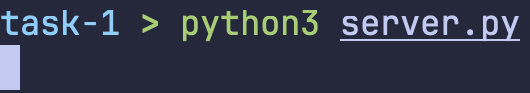
\includegraphics[width=0.5\textwidth]{images/task-1/server-waits.png}
  \caption{Ожидание сервером запроса от клиента}
  \label{fig:task-1:server-waits}
\end{figure}

\begin{figure}[H]
  \centering
  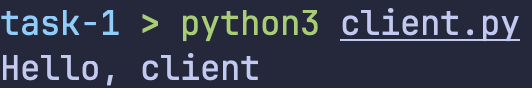
\includegraphics[width=0.5\textwidth]{images/task-1/client-result.png}
  \caption{Ответ клиенту от сервера}
  \label{fig:task-1:client-result}
\end{figure}

\begin{figure}[H]
  \centering
  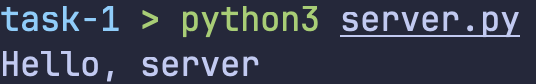
\includegraphics[width=0.5\textwidth]{images/task-1/server-result.png}
  \caption{Ответ серверу от клиента}
  \label{fig:task-1:server-result}
\end{figure}

\subsection*{Задание №2}

В данном задании необходимо реализовать клиентскую и серверную часть приложения.
Клиент запрашивает у сервера выполнение математической операции, параметры,
которые вводятся с клавиатуры. Сервер обрабатывает полученные данные и
возвращает результат клиенту. В соответствии с порядковым номером в журнале,
необходимо реализовать приложение, вычисляющее длину гипотенузы по теореме
Пифагора.

Основной код для данного задания был взят из задания №1. Исходный код сервера и
клиента находится в приложениях \ref{app:task-2:server.py} и
\ref{app:task-2:client.py} соответственно. У клиента теперь вместо сообщения
<<Hello, server>> отправляется сообщение, содержащее два числа разделенных
пробелом. У сервера логика изменилась похожим образом: теперь сервер принимает
эти два числа, вычисляет длину гипотенузы и отправляет ее клиенту.

При запуске сервер сначала ожидает запроса от клиента (рис.
\ref{fig:task-2:server-waits}). После установления соединения, он принимает
полученные числа и отправляет результат клиенту (рис.
\ref{fig:task-2:client-result}).

\begin{figure}[H]
  \centering
  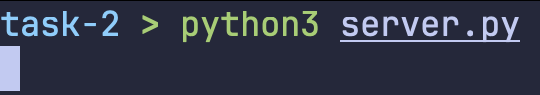
\includegraphics[width=0.5\textwidth]{images/task-2/server-waits.png}
  \caption{Ожидание сервером запроса от клиента}
  \label{fig:task-2:server-waits}
\end{figure}

\begin{figure}[H]
  \centering
  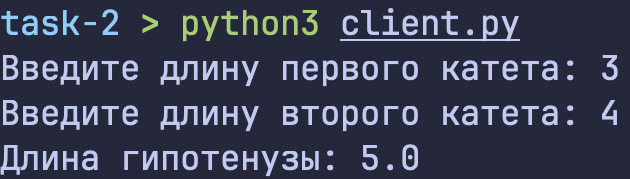
\includegraphics[width=0.5\textwidth]{images/task-2/client-result.png}
  \caption{Ответ клиенту от сервера}
  \label{fig:task-2:client-result}
\end{figure}

\subsection*{Задание №3}

В данном задании необходимо реализовать серверную часть приложения. Клиент
подключается к серверу. В ответ клиент получает http-сообщение, содержащее
html-страницу, которую сервер подгружает из файла index.html.

Получившийся сервер, как и в предыдущих заданиях, использует библиотеку socket.
Теперь, вместо отправления простого текстового сообщения, клиент получает
HTTP-ответ. В данном случае использовались следующие заголовки:
\begin{itemize}
  \item \textbf{Content-Type: text/html} --- для обозначения, что полученные
  данные являются HTML-страницей;
  \item \textbf{Content-Length: N} --- длина полученных данных;
  \item \textbf{Connection: close} --- сообщение о том, что соединение нужно
  закрыть.
\end{itemize}
Полезные данные, т. е. HTML-страница, подгружается из файла index.html. На рис.
\ref{fig:task-3:curl} изображен результат выполнения HTTP-запроса к серверу с
помощью утилиты curl. Как видно, после выполнения запроса сервер прислал
HTML-страницу, как и ожидалось. Если открыть браузер по адресу localhost:3000,
то будет загружена страница, изображенная на рис. \ref{fig:task-3:browser}.
Исходный код сервера находится в приложении \ref{app:task-3:server.py}.

\begin{figure}[H]
  \centering
  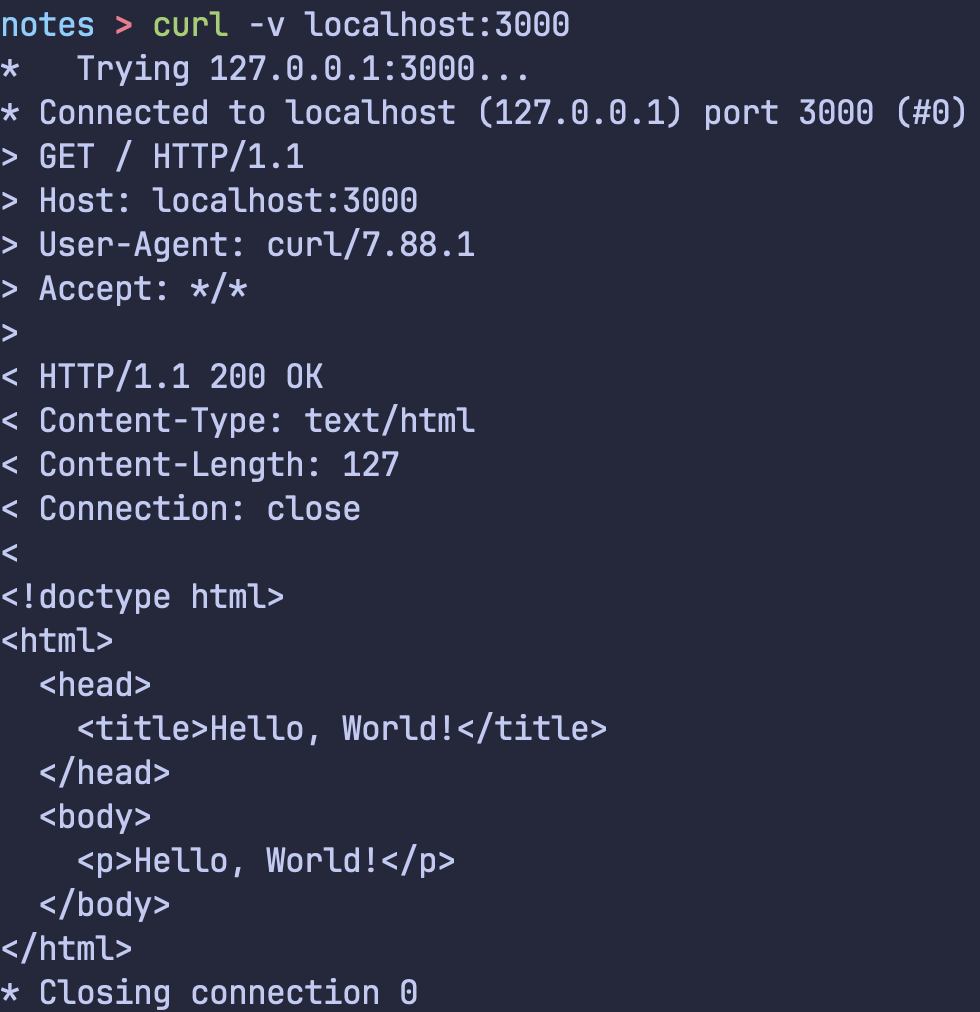
\includegraphics[width=0.7\textwidth]{images/task-3/curl.png}
  \caption{Результат выполнения HTTP-запроса к серверу}
  \label{fig:task-3:curl}
\end{figure}

\begin{figure}[H]
  \centering
  \fbox{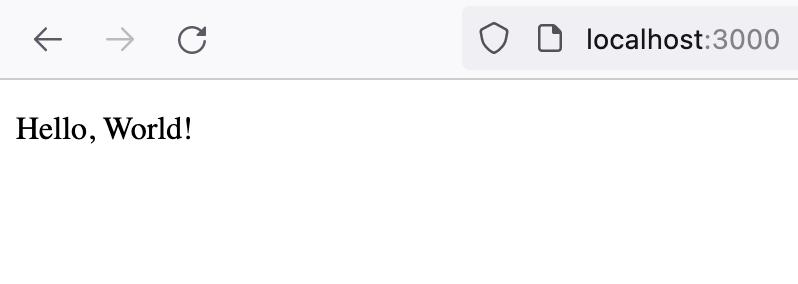
\includegraphics[width=0.8\textwidth]{images/task-3/browser.png}}
  \caption{Страница в браузере}
  \label{fig:task-3:browser}
\end{figure}

\subsection*{Задание №4}

В данном задании необходимо реализовать многопользовательский чат. При
выполнении данного задания также использовалась библиотека socket для реализации
сетевого взаимодействия. Также использовалась библиотека threading для создания
новых потоков. Она была нужна для того, чтобы сервер мог принимать и
обрабатывать запросы сразу от нескольких клиентов. Также threading
использовалась и для реализации клиентской части. Она использовалась для того,
чтобы клиент мог получать новые сообщения сразу же, как только они появились, а
не только тогда, когда клиент отправляет сообщения.

Сервер реализован следующим образом. Он, подобно предыдущим заданиям,
прослушивает входящие соединения. В случае, если соединение установлено,
создается новый поток с помощью библиотеки threading. В этом потоке происходит
считывание получаемых сообщений и рассылка этих сообщений на другие клиенты.
Исходный код сервера находится в приложении \ref{app:task-4:server.py}.

Клиент устроен следующим образом. Он считывает у пользователя его имя и
подключается к серверу. После подключения пользователь создает дополнительный
поток для получения и вывода новых сообщений, принимаемых от сервера. Далее
клиент начинает считывать пользовательский ввод и отправлять его на сервер.
Исходный код клиента находится в приложении \ref{app:task-4:client.py}.

При запуске клиента пользователю сначала предлагается ввести его имя (рис.
\ref{fig:task-4:username}). После этого пользователь может начать вводить
сообщения. После отправки сообщения первым пользователем (рис.
\ref{fig:task-4:send-message}), второй сразу же увидит его у себя на экране
(рис. \ref{fig:task-4:receive-message}).

\begin{figure}[H]
  \centering
  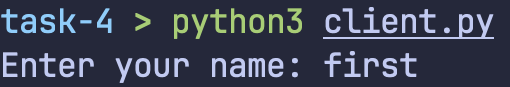
\includegraphics[width=0.5\textwidth]{images/task-4/username.png}
  \caption{Ввод имени подключившегося пользователя}
  \label{fig:task-4:username}
\end{figure}

\begin{figure}[H]
  \centering
  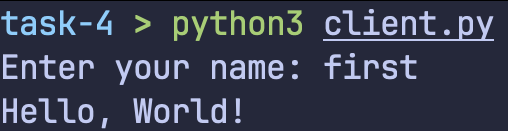
\includegraphics[width=0.5\textwidth]{images/task-4/send-message.png}
  \caption{Отправка сообщения первым пользователем}
  \label{fig:task-4:send-message}
\end{figure}

\begin{figure}[H]
  \centering
  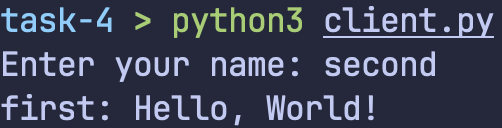
\includegraphics[width=0.5\textwidth]{images/task-4/receive-message.png}
  \caption{Получение сообщения вторым клиентом}
  \label{fig:task-4:receive-message}
\end{figure}

\section{Вывод}

В ходе выполнения лабораторной работы я овладел практическими навыками и
умениями реализации веб-серверов и использования сокетов.

\newpage

\appendix

\titleformat{\section}[display]
{\normalfont\bfseries}
{\centering Приложение\ \thesection}
{0pt}{\centering}
\renewcommand{\thesection}{\Asbuk{section}}

\section{Исходный код сервера задания №1}
\label{app:task-1:server.py}

\begin{code}
  \inputminted{python}{../task-1/server.py}
\end{code}

\newpage

\section{Исходный код клиента задания №1}
\label{app:task-1:client.py}

\begin{code}
  \inputminted{python}{../task-1/client.py}
\end{code}

\newpage

\section{Исходный код сервера задания №2}
\label{app:task-2:server.py}

\begin{code}
  \inputminted{python}{../task-2/server.py}
\end{code}

\newpage

\section{Исходный код клиента задания №2}
\label{app:task-2:client.py}

\begin{code}
  \inputminted{python}{../task-2/client.py}
\end{code}

\newpage

\section{Исходный код сервера задания №3}
\label{app:task-3:server.py}

\begin{code}
  \inputminted{python}{../task-3/server.py}
\end{code}

\newpage

\section{Исходный код сервера задания №4}
\label{app:task-4:server.py}

\begin{code}
  \inputminted{python}{../task-4/server.py}
\end{code}

\newpage

\section{Исходный код клиента задания №4}
\label{app:task-4:client.py}

\begin{code}
  \inputminted{python}{../task-4/client.py}
\end{code}

\end{document}
